\documentclass{ccr15}
% PACKAGES ---------------------------------------------------------------
\usepackage{amsfonts,amsmath,graphicx,subfigure}
\usepackage{listings}
\usepackage{url}
\usepackage{color}
% ADD YOUR OWN PACKAGES HERE ---------------------------------------------
%\usepackage{someotherpackage}
% DEFINITIONS ------------------------------------------------------------
% ADD YOUR OWN DEFINITIONS HERE ------------------------------------------
\definecolor{hellgelb} {rgb}{1.0,1.0,0.8}   % background color for C++ listings
\definecolor{darkgreen}{rgb}{0.0,0.2,0.13}
\lstset{
  backgroundcolor=\color{hellgelb},
  basicstyle=\ttfamily\tiny,
  breakautoindent=true,
  breaklines=true,
  captionpos=b,
  columns=flexible,
  commentstyle=\color{darkgreen},
  extendedchars=true,
  float=hbp,
  frame=single,
  identifierstyle=\color{black},
  keywordstyle=\color{blue},
  numbers=none,
  numberstyle=\tiny,
  showspaces=false,
  showstringspaces=false,
  stringstyle=\color{purple},
  tabsize=2,
}
% BE SURE TO PREFACE LABEL WITH YOUR OWN INITIALS (ZAB in this example) --
% This controls the table-of-contents entry in the proceedings. Edit it
% to include your article title followed by the authors' names, as shown.
\addcontentsline{toc}{chapter}{Performance Portable High Performance Conjugate Gradient Benchmark\\
{\em Z.B.\ Student and I.D.\ Mentor and S.R \ Mentor}}
\pagestyle{myheadings}
\thispagestyle{plain}
% This gives the running head. Usually you list a shortened version of
% your article title (unless it's already very short) along with
% the author's names, as shown.
\markboth{Performance Portable High Performance Conjugate Gradient Benchmark}{Z.B.\ Student and I.D.\ Mentor and S.R \ Mentor}
% Put your article title in here
\title{Performance Portable High Performance Conjugate Gradient Benchmark}
% List each author, their affiliation, and their e-mail address, as shown.
\author{Zachary A.\ Bookey\thanks{Saint John's University, zabookey@csbsju.edu} \and Irina P.\ Demeshko\thanks{Sandia National Laboratories,
ipdemes@sandia.gov} \and Sivasankaran Rajamanickam\thanks{Sandia National Laboratories, srajama@sandia.gov}\and Michael A. Heroux\thanks{Sandia National Laboratories, maherou@sandia.gov}}
\begin{document}
\maketitle
% Include your abstract here.
\begin{abstract}
The High Performance Conjugate Gradient Benchmark (HPCG) is an international project to create a
more appropriate benchmark test for the world's largest computers. The current LINPACK benchmark,
which is the standard for measuring the performance of the top 500 fastest computers in the
world, is moving computers in a direction that is no longer beneficial to many important
parallel applications. In this project we are developing a version of HPCG, using the Kokkos
package in Trilinos. Kokkos can be optimally executed across several distinct high
performance computing architectures. 
%Irina comment: the last sentence of the abstract should outline the main goal/result of of this work. So we might want to change it.
This new code demonstrates an efficient programming
approach that can be adopted by other programmers to write portable high performance software.
\end{abstract}

\section{Introduction}

After generations of using the High Performance Linpack (HPL), or Top 500, benchmark \cite{ZAB:Top500} to measure the
performance of large computers it became necessary to use another benchmark to help better the
direction that super computers were headed to more accurately reflect the types of applications
that these machines were running.

HPL is a simple program that factors and solves a large dense system of linear equations using
Gaussian Elimination with partial pivoting.
While dense matrix - matrix multiplication and related kernels are commonly used in scientific applications,
they are not representative of all the operations usually performed in scientific computing:
computations with lower computation-to-data-access ratios(computational intensity) and with
irregular memory access are also very common.

The High Performance Conjugate Gradient (HPCG)\cite{ZAB:TechHPCG}\cite{ZAB:TechHPCG2} was created to fill the gap that HPL had created.
HPCG uses a preconditioned conjugate gradient to solve a system of equations, that executes both
dense computations with high computational intensity and computations with low computational intensity such as sparse matrix-matrix multiplications.

Original HPCG benchmark doesn't exploit full parallelism available on existing supercomputers which makes it unfair to use HPCG for performance measurement on architectures with accelerators/co-processors.
The goal of our project was to create a performance portable version of HPCG that gives reasonable performance on all existing supercomputers. 
We choose  Kokkos\cite{ZAB:Kokkos} library from Trilinos\cite{ZAB:Trilinos} as a tool to provide performance portability in HPCG code.

% Irina comment: I think we can add related work here

\section{HPCG}

HPCG is a new and
upcoming benchmark test to rank the world's largest computers. On top
of solving a large system of equations, HPCG also features a more irregular data access pattern
so that data access affects results as well as matrix computations.

HPCG begins by creating a symmetric positive definite matrix and it's corresponding multigrid
to be used in the preconditioning phase. For the preconditioner it uses a Symmetric Gauss-Seidel
forward sweep and back sweep to solve the lower and upper triangular matrices. For the actual
solve of $A x = b$, HPCG uses the conjugate gradient method after the preconditioning phase.
HPCG runs in seven major phases.
\begin{enumerate}
\item \textbf{Problem Setup:} This is the beginning of HPCG and is where we construct the
geometry that is used to generate the problem. HPCG generates a symmetric, positive definite,
sparse matrix with up to 27 nonzero entries per row depending on the local location of the row.
\item \textbf{Validation Testing:} This portion of the program is to make sure any changes
made produce valid results. Specifically it checks to make sure that both the unpreconditioned
and preconditioned conjugate gradient converge in around 12 and 2 iterations respectively. It
also makes sure that after performing both a sparse matrix vector multiplication and a symmetric
Gauss-Seidel sweep that we preserve symmetry by using two randomly filled vectors and
performing simple operations that should be zero due to the nature of our symmetric matrix A.
\item \textbf{Reference Sparse Matrix Vector Multiplication and Multigrid Timing:} This
portion of the code times how long it takes to perform the reference versionts of SPMV and
Symmetric Gauss-Seidel.
\item \textbf{Reference Conjugate Gradient Timing:} Here we run 50 iterations of the reference
version of the conjugate gradient method and record the resulting residual. This residual must be
attained by the optimized version of conjugate gradient no matter how many iterations are
required.
\item \textbf{Optimized Conjugate Gradient Setup:} Runs one set of the optimized conjugate
gradient and determines the number of iterations required to reach the residual found before.
Then figures out how mamy times to reach the desired residual to fill in the requested benchmark
time.
\item \textbf{Optimized Conjugate Gradient Timing:} Runs the optimized conjugate gradient the
required amount of times. Records time for each timed section to report out later.
\item \textbf{Report Results:} Writes out log files for debugging and creates the .yaml file
to display the results which can then be submitted if all the requirements are met.
\end{enumerate}
HPCG gives you the option to run with MPI, OpenMP, both, or in serial. Running with MPI adds an
extra dimension to the problem and requires processes to exchange values on their borders to
perform. This results in a tradeoff between more overhead and more parallelism.
\section{Kokkos}
As computer architectures differ in their features for best parallel performance it has
become increasingly difficult to write code that will perform well across many different types of
architectures. One solution to this problem is the C++ package, Kokkos. Kokkos acts as a wrapper
around your code to allow you to specify at compile time where and how you want to run your
application. Kokkos executes computational kernels in fine-grain data parallel within an 
\texttt{Execution space}.
Currently Kokkos supports the following \texttt{Execution spaces}:
\begin{itemize}
\item \texttt{Serial}
\item \texttt{PThreads}\cite{ZAB:PThreads}
\item \texttt{OpenMP}\cite{ZAB:OpenMP}
\item \texttt{Cuda}\cite{ZAB:CUDA}
\end{itemize}

Kokkos has two main features: \texttt{Kokkos::View} polymorphic Multidimensional  Arrays and parallel dispatch.
  \texttt{Kokkos::View} is essentially a wrapper around
an array of data that gives you the option to specify which \texttt{Execution space} you want to store the
data on and allows you to choose what sort of memory access traits you wish this data to have.
\texttt{Kokkos::View}  also handle their own memory management via reference counting so that the view
automatically deallocates itself when all of the variables that reference it go out of scope,
thus making memory management much simpler across multiple devices.

There are three main parallel dispatch operations in Kokkos: \texttt{parallel\_for,}  \texttt{parallel\_reduce}, and \texttt{parallel\_scan}. 
All of these serve their own purpose and act as wrappers over how you would execute a section of 
code in parallel over the respective \texttt{Execution space}. 
For all of the data parallel executions kernels you initiate the kernel by passing in a functor 
that performs the desired parallel operation, such as from host to device.

\texttt{Parallel\_for} is simply a generic for loop that will run all of the context of the loop in
parallel. This works well for parallel kernels like vector addition. 

\texttt{Parallel\_reduce} is for
simultaneously updating a single value, this function guarantees that you avoid race conditions
with the updated values. \texttt{Parallel\_reduce} works well for parallel kernels like finding the dot
product of two vectors. 

\texttt{Parallel\_scan} is for taking a view and creating a running sum of values
to replace the values of the view. Although \texttt{parallel\_scan} is useful it was only really needed
for setup phases in our HPCG.

%Irina comment: this explanation is not clear. Could you, please, add more details (we can use some from the Programming guide)
%Zach comment: Is this any better?
Kokkos allows for nested parallelism. This enables us to run up to three level parallelism inside a single kernel.
This happens by creating a league of thread teams so that each team of threads has a specified number of threads.
Then we can assign vector lanes to each thread that can run in parallel as well. This allows us to call a parallel 
kernel on the league and then another parallel kernel on the teams and finally a parallel kernel on the vector 
lanes of the thread. Depending on the type of problem you're working on this could introduce unnecessary overhead 
and you'd be better off with one level of parallelism. We'll explore this further in HPCG later.

%Irina comment: we need to change following since we have already implemented this in HPCG.
%Zach comment: Addressed above.

%Although this has not been implemented in our project yet, there are places in our code that
%could and should benefit from nested parallelism and thus we intend to include it at a later
%time.

\section{HPCG + Kokkos}

The goal for our project was to create a version of HPCG that 
produces valid results across many architectures without sacrificing performance.
We believe that Kokkos library is the best available tool to provide performance portability for the C++ code, we choose to refactor HPCG to use it.

General strategy for Kokkos re-factoring includes: 
\begin{itemize}
\item replacement custom data types with Kokkos multidimensional arrays; 
\item replacement the parallel loops with Kokkos parallel kernels; 
\item code optimizations to improve usage of co-processors.
\end{itemize}

% First we needed to rewrite the parallel kernels to use Kokkos parallel kernels, then we needed to restructure 
%all of the code to work with Kokkos views, and finally we needed to make a few optimizations to
%avoid an unecessary amount of memory copying from the host to the device and vice versa.



\subsection{Replacement custom data types with Kokkos multidimensional arrays}

Restructuring the code involved a whole rewrite of HPCG to change how all of the structs stored
their values. We replaced every array that would be used in a parallel kernel with an appropriate
view. Once this was functional we had to go back to some of the compute algorithms and change
how the data was accessed as to not try to access device data from the host or the
other way around.

While restructuring we decided to change how our SparseMatrix stored the data and implemented it
as a sort of overlying structure on top of a Kokkos CSRMatrix. This change required us to again
go back and change how most of our computational kernels worked and created a noticeable increase
in performance. At this point the code was functional across all of Kokkos execution spaces but
took a severe performance hit while trying to run on Cuda. (TODO : Due to host to device copies for sequential kernels? )

\subsection{Replacement the parallel loops with Kokkos parallel kernels}

Re-writing the parallel kernels involved replacing the parallel loops with the correct type of
Kokkos parallel kernel. This part of re-factoring was heavily focused on converting the
computation algorithms into functors and lambdas. Completing this task didn't affect portability
at all and due to some Kokkos restrictions actually caused a slight reduction of performance in
the function ComputeResidual. Other kernels would later have to be changed to accommodate the fact
that data was stored on a device but was being run on the host.

Computing the preconditioner using a symmetric Gauss-Seidel was initially done in serial and thus
moving to Kokkos required us to copy memory from the device to the host every time we ran it,
which was the reason performance was lost. We tried implementing many different ways to perform
a sweep of symmetric Gauss-Seidel in parallel to eliminate the need of copying data. We
implemented an \emph{inexact solve}, a \emph{level solve}, and a \emph{coloring algorithm}.
%Irina comment: do we have any references for inexact solve, a level solve, and a coloring algorithm.
%Zach comment: This is a Siva question. I have the book he lent me and I'll cite that, otherwise I don't know
%where these algorithms came from.


The \emph{inexact solve} works by performing a few triangular matrix solves. We split our matrix $A$ into
parts $L$, $U$, and $D$ where $L$ is the lower triangular matrix including the diagonal, $U$ is the upper
triangular matrix including the diagonal and $D$ is the diagonal. The \emph{inexact solve} is done by solving three
different equations. Given our problem $A x = b$, to simulate a symmetric Gauss-Seidel sweep we solve
$L z = b$ then $D w = z$ and finally $U x = w$. All of these solves are done using a parallel Jacobi solve.
Although this version of symmetric Gauss-Seidel is run in parallel and avoid all device to host memory
copies it still performs slowly since each Jacobi solve needs to be run a certain number of sweeps depending
on problem density and results in more parallel kernels being launched than is ideal.

Our \emph{level solve} algorithm splits our matrix $A$ into parts $L$, $U$, and $D$ where $L$ is the
lower triangular part of $A$ that includes the diagonal, $U$ is similar to $L$ since it is just
the upper triangular part of $A$ that includes the diagonal. $D$ is just the diagonal of A. For
this algorithm we introduce another data structure, levels, to our SparseMatrix that stores all 
of the data needed for sorting the matrix. When we optimize the problem we find dependencies in
solving for $L$ and sort based on those dependencies in a way that a row will only be solved if
all of it's dependencies have been solved. We repeat this process for solving for $A$ and store
all of this data into levels. Now when we compute our Symmetric Gauss-Seidel we solve just like
we do for the inexact solve except we start by solving for the rows in level 1 in parallel and
then the rows in level 2 in parallel and repeat until we solve all of our levels. In the end we
have a Symmetric Gauss-Seidel that has introduced a deal of parallelism and performs well
compared to the original implementation.

At the time of writing our \emph{coloring algorithm} is not fully implemented. We are in the process of finishing it to provide it as part of HPCG+Kokkos
implementation.
The algorithm works by coloring our matrix $A$ so that all rows
with a certain color have no dependencies on one another. This way we can run a sweep of symmetric
Gauss-Seidel in parallel over each color. While similar to the level solve, this method requires more iterations
to converge due to the fact that although no two rows in the same color depend on each other it is likely
that they depend on a row in a color that will be solved in a later iteration.

\section{Performance evaluation}
We evaluate performance for our implementation of the HPCG code on our Compton and Shannon testbed clusters. Compton is used for Intel Xeon and Intel Xeon Phi tests, and Shannon is used for NVIDIA Kepler (K20x) tests. Testbed configuration details are given in Table \ref{testbeds}. Note that in these configurations device refers to a dual socket Xeon node, a single Xeon Phi, and a single Kepler GPU respectively.
Results presented in this paper are for pre-production Intel Xeon Phi co-processors (codenamed Knights Corner) and pre-production versions of Intel{'}s Xeon Phi software stack. Performance and configuration of the co-processors may be different in final production releases.

\begin{table}[h]
\centering
\resizebox{2.7in}{!}{
\begin{tabular}{lll}
\hline    
 Name & Compton & Shannon      \\
 \hline    
 \\
 Nodes & 32 & 32  \\
\\
 CPU &2� Intel E5-2670 HT-on &2� Intel E5-2670 HT-off  \\
 \\
 Co-Processor &2� Intel Xeon Phi 57c  &2� K20x ECC on  \\
 & 1.1 GHz &\\
 Memory  &64 GB &  128 GB  \\
 \\
 Interconnect  & QDR IB &  QDR IB  \\
 \\
 OS  & RedHat 6.1 & RedHat 6.2   \\
 \\
 Compiler & ICC 13.1.2 & GCC 4.8.2+CUDA 6.5   \\
 \\
 MPI & IMPI 4.1.1.036  & MVAPICH2 1.9  \\
 \\
 Other &MPSS 2.1.3653-8 & Driver: 319.23  \\
 \\
 \hline    
\end{tabular}}
 \caption{Configurations of testbed clusters}
 \label{testbeds}
\end{table}

Comparing different variations of the preconditioner requires us to consider different problem sizes
since some of our implementations will perform better on larger more sparse matrices than they will
on smaller and denser matrices. 

As you can see in Table \ref{SYMGS16} the standard version of symmetric Gauss-Seidel performs
best since the level solve and the inexact solve only have limited parallelism. This is due to
the fact that there aren't enough non-dependent rows to provide sufficient parallelism on each
level and the inexact solve needs 18 iterations to get a solution for each triangular matrix that
is close enough to the exact solution to maintain symmetry.

\begin{table}[h]
\begin{center}
\begin{tabular}{|c||c|c|c|}
\hline
 & Standard SYMGS & Level Solve & Inexact Jacobi Solve \\
 \hline \hline
 Cuda (Shannon) & 0.408776 & 0.0634977 & 0.091606 \\
 \hline
 OpenMP (Shannon) & 1.67202 & 0.233525 & 0.295145 \\
 \hline
 Serial (Shannon) & 1.46676 & 0.22152 & 0.269744 \\
 \hline
\end{tabular}
\caption{SYMGS on Problem Size $16^3$}
\label{SYMGS16}
\end{center}
\end{table}

As seen in Table \ref{SYMGS64} the level solve begins to become the optimal preconditioner. This
is similar to the issue with size $16^3$ where now our matrix is large and sparse enough that
the level solve starts to see an increased amount of parallelism. The inexact method still lags
behind since even though our matrix is less dense it still needs 12 Jacobi iterations to have
a solution exact enough to pass the symmetry test.

\begin{table}[h]
\begin{center}
\begin{tabular}{|c||c|c|c|}
\hline
& Standard SYMGS & Level Solve & Inexact Jacobi Solve \\
\hline \hline
Cuda (Shannon) & 0.64954 & 0.720434 & 0.560632 \\
\hline
OpenMP (Shannon) & 1.76462 & 2.42687 & 0.97734 \\
\hline
Serial (Shannon) & 1.45816 & 1.56839 & 0.485523 \\
\hline
\end{tabular}
\caption{SYMGS on Problem Size $64^3$}
\label{SYMGS64}
\end{center}
\end{table}

Table \ref{SYMGS128} shows us still that level solve is our most optimal preconditioner for
similar reasons as stated before. However it makes sense to note that the inexact solve is
steadily increasing performance as we our problem size increases. With a problem size of $128^3$
we only need 5 jacobi iterations to achieve a near exact solution to each triangular solve.

\begin{table}[h]
\begin{center}
\begin{tabular}{|c||c|c|c|}
\hline
& Standard SYMGS & Level Solve & Inexact Jacobi Solve \\
\hline \hline
Cuda (Shannon) & 0.660526 & 2.1373 & 1.39231 \\
\hline
OpenMP (Shannon) & 1.82678 & 4.19081 & 1.84878 \\
\hline
Serial (Shannon) & 1.49575 & 2.18794 & 0.810011 \\
\hline
\end{tabular}
\caption{SYMGS on Problem Size $128^3$}
\label{SYMGS128}
\end{center}
\end{table}

In Table \ref{SYMGS192} we tested our preconditioning algorithms on a problem size of $192^3$. As
expected our standard Gauss-Seidel performed at the same level as before and our level solve
starts to slow down its performance increases. The inexact solve left us with some abnormally
high results that remained valid. For executing on OpenMP we witnessed results of 100+ GFLOPS
and for Cuda we found high 90's. We are still investigating what may have caused these results.

\begin{table}[h]
\begin{center}
\begin{tabular}{|c||c|c|c|}
\hline
& Standard SYMGS & Level Solve & Inexact Jacobi Solve \\
\hline \hline
Cuda (Shannon) & 0.659346 & 2.89654 & ??? \\
\hline
OpenMP (Shannon) & 1.842 & 4.858 & ??? \\
\hline
Serial (Shannon) & 1.5048 & 2.37896 & ??? \\
\hline
\end{tabular}
\caption{SYMGS on Problem Size $192^3$}
\label{SYMGS192}
\end{center}
\end{table}

Now we're going to look at how each preconditioning algorithm performs overall on each execution
space.

As seen in Fig \ref{Vanilla} the vanilla symmetric Gauss-Seidel is dominant on the non-cuda
execution spaces. This has to do with the fact every time this method is called we had to run
a lot of memory copies between the host and device. When we aren't using Cuda all of our memory
is located in one space and thus the memory copying is avoided and we don't see a huge
performance hinderance.

\begin{figure}[H]
  \centering
  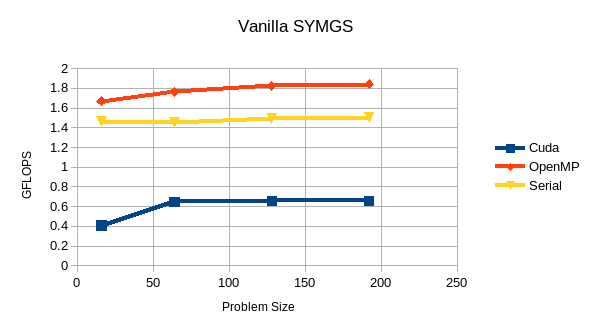
\includegraphics[width=10cm]{plots/ZAB-VanillaSYMGS.png}
  \caption{Plot of GFLOPS for Vanilla SYMGS on each execution space.}
	\label{Vanilla}
\end{figure}

In Fig \ref{Level} the results between execution spaces while using the level solve
preconditioning method vary quite a bit. First, notice that there is a trend with the results and
it appears that our max performance received from this preconditioner starts to taper off. With
this trend in mind it appears that OpenMP will acheive better performance using this
preconditioner than Cuda. However this could be because we haven't done much cuda optimizaitons
in terms of memory.

\begin{figure}[H]
	\centering
	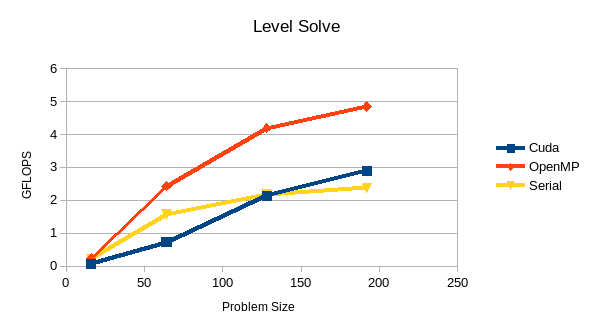
\includegraphics[width=10cm]{plots/ZAB-LevelSolve.png}
	\caption{Plot of GFLOPS for level solve on each execution space.}
	\label{Level}
\end{figure}

Looking at Fig \ref{Inexact} it seems we have a trend that increases our performance based on
problem size. I'm confident this has to do with the fact that when our problem size is larger our
matrix is less dense and so we need less jacobi iterations to produce an answer exact enough to
pass the symmetry tests. However we opt to leave out problem size $192^3$ due to the abnormal
results mentioned before.

\begin{figure}[H]
	\centering
	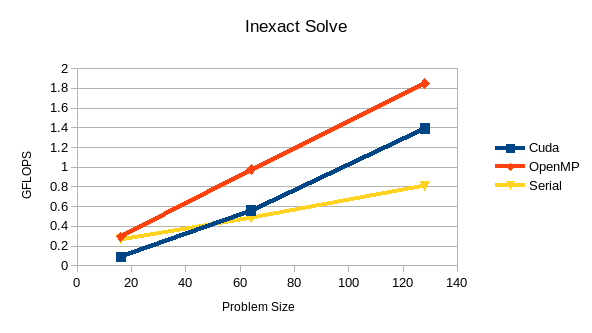
\includegraphics[width=10cm]{plots/ZAB-InexactSolve.png}
	\caption{Plot of GFLOPS for inexact solve on each execution space.}
	\label{Inexact}
\end{figure}

\subsection{Optimizations}
Aside from the symmetric Gauss-Seidel optimizations already made, we are looking to further these
optimizations in the future by exploiting hierarchical parallelism. For example, in the \emph{inexact
solve} we can implement a three level parallelism technique that breaks our rows into chunks that 
a team of threads each gets assigned. Now our teams of threads work on our chunk while in
parallel we perform the matrix vector computation in parallel using the threads in the team. A
near identical method can be applied to our \emph{level solve algorithm} but since the level solve deals
with fewer rows at a time we won't see as much of a performance increase in here. We're confident
that these aren't the only places that can benefit from hierarchical parallelism and we plan to
explore these options at a later time.
%Irina comment: should we add a code example for the hierarchical parallelism?
%Zach comment: I'll find a way to add a code snippet of nested parallelism when I'm in the office.

We have started implementing some nested parallelism into our inexact solve method for symmetric gauss-seidel.
And looking at figures \ref{vlength_cuda} and \ref{vlength_openmp} it is clear that Cuda receives a huge benefit
from this as it allows us to finely tune how we want to parallelize this method. This nested implementation works as described
above and for our figures it chooses chunks of size $n$ for a problem of size $n^3$. This assures us that we 
actually work with every row in our matrix and gives us decent results. We encountered an issue as our threads
were only able to launch 4 vector lanes max and the kernel itself would not run if we tried to launch more. These results
are highly preliminary as we intend to explore what the optimal number of rows per chunk is and as we figure out
why we're only allowed to launch 4 vector lanes from a thread.

\begin{table}[h]
\begin{center}
\begin{tabular}{|c||c|c|c|}
\hline
& Vector Length 1 & Vector Length 2 & Vector Length 4 \\
\hline
$N=16$ & 0.087516 & 0.0857736 & 0.0834751 \\
\hline
$N=64$ & 0.611932 & 1.41309 & 1.17325 \\
\hline
$N=128$ & 1.2713 & 3.51299 & 4.07047 \\
\hline
\end{tabular}
\caption{Nested Parallelism Using Cuda and Specified Vector Length on Problem Size $N^3$}
\label{VLC}
\end{center}
\end{table}

\begin{table}[h]
\begin{center}
\begin{tabular}{|c||c|c|c|}
\hline
& Vector Length 1 & Vector Length 2 & Vector Length 4 \\
\hline
$N=16$ & 0.110544 & 0.111938 & 0.111116 \\
\hline
$N=64$ & 0.50259 & 0.502229 & 0.495932 \\
\hline
$N=128$ & 1.09584 & 1.11385 & 1.11723 \\
\hline
\end{tabular}
\caption{Nested Parallelism Using OpenMP and Specified Vector Length on Problem Size $N^3$}
\label{VLO}
\end{center}
\end{table}

Below is a code snippet that demonstrates how we used Kokkos heirarchial parallelism in the lower trisolve
kernel for the inexact solve version of the symmetric Gauss-Seidel.
\lstset{language=[Visual]C++}
\lstinputlisting{plots/HeirarchialSnippet.cpp}

\begin{figure}[H]
	\centering
	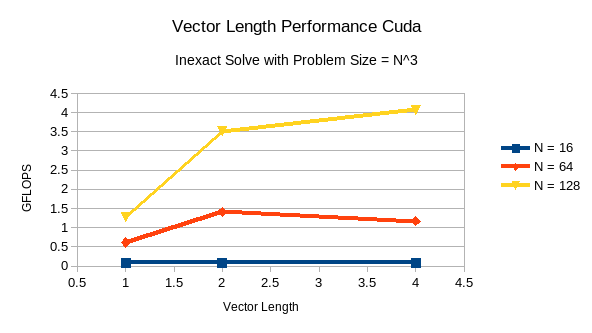
\includegraphics[width=10cm]{plots/ZAB-VectorLengthCuda.png}
	\caption{Plot of GFlops for diffenet vector lengths, used in inexact solve, across problem sizes in Cuda}
	\label{vlength_cuda}
\end{figure}

\begin{figure}[H]
	\centering
	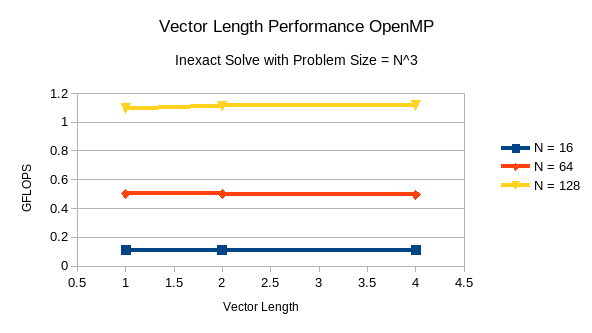
\includegraphics[width=10cm]{plots/ZAB-VectorLengthOpenMP.png}
	\caption{Plot of GFlops for different vector lengths, used in inexact solve, across problem sizes in OpenMP}
	\label{vlength_openmp}
\end{figure}

\section{Conclusion}
In the end we have worked towards creating a version of HPCG that works alongside the Kokkos
package found in Trilinos. This version of HPCG will be a useful for being able to run the reference
version of HPCG out of the box and not need to configure the code to be compatible with the
specific machine being benchmarked.

Our work here is not completed but we have made great headway on this project and currently have
code that produces similar results across all of the Kokkos execution spaces. In the future we want to
fix a few performance bottlenecks and utilize hierarchical parallelism to fully take advantage of Kokkos
kernels.We also want to fix our coloring algorithm for the symmetric Gauss-Seidel so we can choose at
compile time which algorithm to use for preconditioning. It will be interesting to compare performance
between all of our preconditioning algorithms.
\section{Acknowledgments}
Sandia National Laboratories is a multi-program laboratory managed and operated by Sandia Corporation, a wholly owned subsidiary of Lockheed Martin Corporation, for the US Department of Energy{'}s National Nuclear Security Administration under contract DE-AC04-94AL85000. This paper is cross-referenced at Sandia as SAND

\bibliographystyle{siam}
% Edit the line below to be your first and last names.
%\nocite{ZAB:Mentor05}
\nocite{ZAB:TechHPCG}
\nocite{ZAB:TechHPCG2}
\nocite{ZAB:Kokkos}
\nocite{ZAB:Trilinos}
\nocite{ZAB:Top500}
\nocite{ZAB:CUDA}
\nocite{ZAB:OpenMP}
\nocite{ZAB:PThreads}
\nocite{ZAB:SYMGS}
\bibliography{ZacharyBookey}
% Edit FirstnameLastname below to be your first and last names, but leave the line commented out.
% This line will help me merge bibliographies for the proceedings.
%\documentclass{ccr15}
% PACKAGES ---------------------------------------------------------------
\usepackage{amsfonts,amsmath,graphicx,subfigure}
\usepackage{listings}
% ADD YOUR OWN PACKAGES HERE ---------------------------------------------
%\usepackage{someotherpackage}
% DEFINITIONS ------------------------------------------------------------
% ADD YOUR OWN DEFINITIONS HERE ------------------------------------------
% BE SURE TO PREFACE LABEL WITH YOUR OWN INITIALS (ZAB in this example) --
% This controls the table-of-contents entry in the proceedings. Edit it
% to include your article title followed by the authors' names, as shown.
\addcontentsline{toc}{chapter}{Performance Portable HPCG\\
{\em Z.B.\ Student and I.D.\ Mentor and S.R \ Mentor}}
\pagestyle{myheadings}
\thispagestyle{plain}
% This gives the running head. Usually you list a shortened version of
% your article title (unless it's already very short) along with
% the author's names, as shown.
\markboth{Performance Portable HPCG}{Z.B.\ Student and I.D.\ Mentor and S.R \ Mentor}
% Put your article title in here
\title{Performance Portable HPCG}
% List each author, their affiliation, and their e-mail address, as shown.
\author{Zachary A.\ Bookey\thanks{Saint John's University, zabookey@csbsju.edu} \and Irina P.\ Demeshko\thanks{Sandia National Laboratories,
ipdemes@sandia.gov} \and Sivasankaran Rajamanickam\thanks{Sandia National Laboratories, srajama@sandia.gov}}
\begin{document}
\maketitle
% Include your abstract here.
\begin{abstract}
%Irina comment: we can't use acronyms in abstarct
The High Performance Conjugate Gradients Benchmark is an international project to create a
more appropriate benchmark test for the world's largest computers. The current LINPACK benchmark,
which is the standard for measuring the performance of the top 500 fastest computers in the
world, is moving computers in a direction that is no longer beneficial to many important
parallel applications. In this project we are developing a version of HPCG, using the Kokkos
package found in Trilinos, that can be optimally executed across several distinct high
performance computing architectures. This new code demonstrates an efficient programming
approach that can be adopted by other programmers to write portable high performance software.
\end{abstract}
\section{Introduction}

After generations of using the High Performance Linpack (HPL) benchmark to measure the
performance of large computers it became necessary to use another benchmark to help better the
direction that super computers were headed to more accurately reflect the types of applications
that these machines were running.

HPL is a simple program that factors and solves a large dense system of linear equations using
Gaussian Elimination with partial pivoting.
While dense matrix - matrix multiplication and related kernels are commonly used in scientific applications,
they are not representative of all the operations usually performed in scientific computing:
computations with lower computation-to-data-access ratios(computational intensity) and with
irregular memory access are also very common.

The High Performance Conjugate Gradient (HPCG) was created to fill the gap that HPL had created.
HPCG uses a preconditioned conjugate gradient to solve a system of equations, that executes both
dense computations with high computational intensity and computations with low computational intensity such as sparse matrix-matrix multiplications.

Original, MPI-only,  HPCG benchmark doesn't exploit full parallelism available on existing Supercomputers which makes it unfair to use it for performance measurement.
And the goal of our project was to create a performance portable version of HPCG that gives reasonable performance on all existing supercomputers, by using Kokkos library from Trilinos.

% Irina comment: I think we can add related work here


\section{HPCG}
HPCG is a new and
upcoming benchmark test to rank the worlds largest computers. On top
of solving a large system of equations, HPCG also features a more irregular data access pattern
so that data access affects results as well as matrix computations.

HPCG begins by creating a symmetric positive definite matrix and it's corresponding multi grid
to be used in the preconditioning phase. For the preconditioner it uses a Symmetric Gauss-Seidel
forward sweep and back sweep to solve the lower and upper triangular matrices. For the actual
solve of $A x = b$, HPCG uses the conjugate gradient method after the preconditioning phase.
HPCG runs in seven major phases.
\begin{enumerate}
\item \textbf{Problem Setup:} This is the beginning of HPCG and is where we construct the
geometry that is used to generate the problem. HPCG generates a symmetric, positive definite,
sparse matrix with up to 27 nonzero entries per row depending on the local location of the row.
\item \textbf{Validation Testing:} This portion of the program is to make sure any changes
made produce valid results. Specifically it checks to make sure that both the unpreconditioned
and preconditioned conjugate gradient converge in around 12 and 2 iterations respectively. It
also makes sure that after performing both a sparse matrix vector multiplication and a symmetric
Gauss-Seidel sweep that we preserve symmetry by using two pseudorandomly filled vectors and
performing simple operations that should be zero due to the nature of our symmetric matrix A.
\item \textbf{Reference Sparse Matrix Vector Multiplication and Multigrid Timing:} This
portion of the code times how long it takes to perform the reference versionts of SPMV and
Symmetric Gauss-Seidel.
\item \textbf{Reference Conjugate Gradient Timing:} Here we run 50 iterations of the reference
version of the conjugate gradient method and record the resulting residual. This residual must be
attained by the optimized version of conjugate gradient no matter how many iterations are
required.
\item \textbf{Optimized Conjugate Gradient Setup:} Runs one set of the optimized conjugate
gradient and determines the number of iterations required to reach the residual found before.
Then figures out how mamy times to reach the desired residual to fill in the requested benchmark
time.
\item \textbf{Optimized Conjugate Gradient Timing:} Runs the optimized conjugate gradient the
required amount of times. Records time for each timed section to report out later.
\item \textbf{Report Results:} Writes out log files for debugging and creates the .yaml file
to display the results which can then be submitted if all the requirements are met.
\end{enumerate}
HPCG gives you the option to run with MPI, OpenMP, both, or in serial. Running with MPI adds an
extra dimension to the problem and requires processes to exchange values on their borders to
perform. This results in a tradeoff between more overhead and more parallelism.
\section{Kokkos}
As different computer architectures are better with certain applications than others it has
become increasingly difficult to write code that will perform well across many different types of
architectures. One solution to this problem is the C++ package, Kokkos. Kokkos acts as a wrapper
around your code to allow you to specify at compile time where and how you want to run your
application. Currently Kokkos supports the following execution spaces:
\begin{itemize}
\item Serial
\item PThreads
\item OpenMP
\item Cuda
\end{itemize}
Kokkos has two main features, views and parallel kernels. A view is essentially a wrapper around
an array of data that gives you the option to specify which execution space you want to store the
data on and allows you to choose what sort of memory access traits you wish this data to have.
Views also handle their own memory management via reference counting so that the view
automatically deallocates itself when all of the variables that reference it go out of scope,
thus making memory management much simpler across multiple devices.

There are three main parallel kernels: parallel\_for, parallel\_reduce, and parallel\_scan. All 
of these serve their own purpose and act as wrappers over how you would execute a section of 
code in parallel over the respective execution space. For all of the parallel kernels you 
initiate the kernel by passing in a functor that performs the desired parallel operation, as of 
host to device.
Parallel\_for is simply a generic for loop that will run all of the context of the loop in
parallel. This works well for parallel kernels like vector addition. Parallel\_reduce is for
simultaneously updating a single value, this function guarantees that you avoid race conditions
with the updated values. Parallel\_reduce works well for parallel kernels like finding the dot
product of two vectors. Parallel\_scan is for taking a view and creating a running sum of values
to replace the values of the view. Although parallel\_scan is useful it was only really needed
for setup phases in our HPCG.
Kokkos allows for nested parallelism that involves creating a league of teams of threads.
With this tool, a developer could launch a parallel\_reduce kernel that uses a parallel\_for to
update some value that later gets added to the value that was initially included to be reduced.
Although this has not been implemented in our project yet, there are places in our code that
could and should benefit from nested parallelism and thus we intend to include it at a later
time.
\section{HPCG + Kokkos}
The goal for our project was to create a version of HPCG that uses Kokkos features to be able to
produce valid results across many architectures without sacrificing performance. First we needed
to rewrite the parallel kernels to use Kokkos parallel kernels, then we needed to restructure 
all of the code to work with Kokkos views, and finally we needed to make a few optimizations to
avoid an unecessary amount of memory copying from the host to the device and vice versa.
\subsection{Kokkos re-factoring}
Rewriting the parallel kernels involved replacing the parallel loops with the correct type of
Kokkos parallel kernel. This part of re-factoring was heavily focused on converting the
computation algorithms into functors and lambdas. Completing this task didn't affect portability
at all and due to some Kokkos restrictions actually caused a slight reduction of performance in
the function ComputeResidual. Other kernels would later have to be changed to accomodate the fact
that data was stored on a device but was being run on the host.

Restructuring the code involved a whole rewrite of HPCG to change how all of the structs stored
their values. We replaced every array that would be used in a parallel kernel with an appropriate
view. Once this was functional we had to go back to some of the compute algorithms and change
how the data was accessed as to not try to access device data from the host or the
other way around.

While restructuring we decided to change how our SparseMatrix stored the data and implemented it
as a sort of overlying structure on top of a Kokkos CSRMatrix. This change required us to again
go back and change how most of our computational kernels worked and created a noticeable increase
in performance. At this point the code was functional across all of Kokkos execution spaces but
took a severe performance hit while trying to run on Cuda.

Computing the preconditioner using a symmetric Gauss-Seidel was initially done in serial and thus
moving to Kokkos required us to copy memory from the device to the host every time we ran it,
which was the reason performance was lost. We tried implementing many different ways to perform
a sweep of symmetric Gauss-Seidel in parallel to eliminate the need of copying data. We
implemented an inexact solve, a level solve, and a colouring algorithm.

Our level solve algorithm splits our matrix $A$ into parts $L$, $U$, and $D$ where $L$ is the
lower triangular part of $A$ that includes the diagonal, $U$ is similar to $L$ since it is just
the upper triangular part of $A$ that includes the diagonal. $D$ is just the diagonal of A. For
this algorithm we introduce another data structure, levels, to our SparseMatrix that stores all 
of the data needed for sorting the matrix. When we optimize the problem we find dependencies in
solving for $L$ and sort based on those dependencies in a way that a row will only be solved if
all of it's dependencies have been solved. We repeat this process for solving for $A$ and store
all of this data into levels. Now when we compute our Symmetric Gauss-Seidel we solve just like
we do for the inexact solve except we start by solving for the rows in level 1 in parallel and
then the rows in level 2 in parallel and repeat until we solve all of our levels. In the end we
have a Symmetric Gauss-Seidel that has introduced a deal of parallelism and performs well
compared to the original implementation.

\subsection{Performance evaluation result}
%Irina comment: I would remove "Future Work" as a section and just add the contect into conclusion
%\section{Future Work}
\section{Conclusion}
\section{Acknowledgements}
%Irina comment: I'll fill this section later 

%Irina comment: I would remove "Future Work" as a section and just add the contect into conclusion
\section{Conclusion}

\section{Acknowledgements}
%Irina comment: I'll fill this section later

\section{Actual Content}
As we saw in Section 1, we all like chocolate pudding. This is where I wish
\textsf{$\setminus$jargonfill} worked. It would fill the page with meaningless technobabble so I could illustrate this
package. Instead, I'll talk about how to use quotations in latex. "Never use these quotations." ``Always use these,
instead.''
\section{Conclusions}
Herein, we repeat the abstract in past tense.
Unlike many other baked goods, chocolate pudding is subject to a myriad of interesting (and unique) effects on both the
meso and nano scales. Understanding these phenomena is critical, not only to America's restaurant industry, but to
children everywhere. We have examined these effects and have proposed new potential models which accurately capture
the material structure of chocolate pudding.
\bibliographystyle{siam}
% Edit the line below to be your first and last names.
\nocite{ZAB:Mentor05}
\nocite{ZAB:TechHPCG}
\bibliography{ZacharyBookey}
% Edit FirstnameLastname below to be your first and last names, but leave the line commented out.
% This line will help me merge bibliographies for the proceedings.
%\documentclass{ccr15}
% PACKAGES ---------------------------------------------------------------
\usepackage{amsfonts,amsmath,graphicx,subfigure}
\usepackage{listings}
% ADD YOUR OWN PACKAGES HERE ---------------------------------------------
%\usepackage{someotherpackage}
% DEFINITIONS ------------------------------------------------------------
% ADD YOUR OWN DEFINITIONS HERE ------------------------------------------
% BE SURE TO PREFACE LABEL WITH YOUR OWN INITIALS (ZAB in this example) --
% This controls the table-of-contents entry in the proceedings. Edit it
% to include your article title followed by the authors' names, as shown.
\addcontentsline{toc}{chapter}{Performance Portable HPCG\\
{\em Z.B.\ Student and I.D.\ Mentor and S.R \ Mentor}}
\pagestyle{myheadings}
\thispagestyle{plain}
% This gives the running head. Usually you list a shortened version of
% your article title (unless it's already very short) along with
% the author's names, as shown.
\markboth{Performance Portable HPCG}{Z.B.\ Student and I.D.\ Mentor and S.R \ Mentor}
% Put your article title in here
\title{Performance Portable HPCG}
% List each author, their affiliation, and their e-mail address, as shown.
\author{Zachary A.\ Bookey\thanks{Saint John's University, zabookey@csbsju.edu} \and Irina P.\ Demeshko\thanks{Sandia National Laboratories,
ipdemes@sandia.gov} \and Sivasankaran Rajamanickam\thanks{Sandia National Laboratories, srajama@sandia.gov}}
\begin{document}
\maketitle
% Include your abstract here.
\begin{abstract}
%Irina comment: we can't use acronyms in abstarct
The High Performance Conjugate Gradients Benchmark is an international project to create a
more appropriate benchmark test for the world's largest computers. The current LINPACK benchmark,
which is the standard for measuring the performance of the top 500 fastest computers in the
world, is moving computers in a direction that is no longer beneficial to many important
parallel applications. In this project we are developing a version of HPCG, using the Kokkos
package found in Trilinos, that can be optimally executed across several distinct high
performance computing architectures. This new code demonstrates an efficient programming
approach that can be adopted by other programmers to write portable high performance software.
\end{abstract}
\section{Introduction}

After generations of using the High Performance Linpack (HPL) benchmark to measure the
performance of large computers it became necessary to use another benchmark to help better the
direction that super computers were headed to more accurately reflect the types of applications
that these machines were running.

HPL is a simple program that factors and solves a large dense system of linear equations using
Gaussian Elimination with partial pivoting.
While dense matrix - matrix multiplication and related kernels are commonly used in scientific applications,
they are not representative of all the operations usually performed in scientific computing:
computations with lower computation-to-data-access ratios(computational intensity) and with
irregular memory access are also very common.

The High Performance Conjugate Gradient (HPCG) was created to fill the gap that HPL had created.
HPCG uses a preconditioned conjugate gradient to solve a system of equations, that executes both
dense computations with high computational intensity and computations with low computational intensity such as sparse matrix-matrix multiplications.

Original, MPI-only,  HPCG benchmark doesn't exploit full parallelism available on existing Supercomputers which makes it unfair to use it for performance measurement.
And the goal of our project was to create a performance portable version of HPCG that gives reasonable performance on all existing supercomputers, by using Kokkos library from Trilinos.

% Irina comment: I think we can add related work here


\section{HPCG}
HPCG is a new and
upcoming benchmark test to rank the worlds largest computers. On top
of solving a large system of equations, HPCG also features a more irregular data access pattern
so that data access affects results as well as matrix computations.

HPCG begins by creating a symmetric positive definite matrix and it's corresponding multi grid
to be used in the preconditioning phase. For the preconditioner it uses a Symmetric Gauss-Seidel
forward sweep and back sweep to solve the lower and upper triangular matrices. For the actual
solve of $A x = b$, HPCG uses the conjugate gradient method after the preconditioning phase.
HPCG runs in seven major phases.
\begin{enumerate}
\item \textbf{Problem Setup:} This is the beginning of HPCG and is where we construct the
geometry that is used to generate the problem. HPCG generates a symmetric, positive definite,
sparse matrix with up to 27 nonzero entries per row depending on the local location of the row.
\item \textbf{Validation Testing:} This portion of the program is to make sure any changes
made produce valid results. Specifically it checks to make sure that both the unpreconditioned
and preconditioned conjugate gradient converge in around 12 and 2 iterations respectively. It
also makes sure that after performing both a sparse matrix vector multiplication and a symmetric
Gauss-Seidel sweep that we preserve symmetry by using two pseudorandomly filled vectors and
performing simple operations that should be zero due to the nature of our symmetric matrix A.
\item \textbf{Reference Sparse Matrix Vector Multiplication and Multigrid Timing:} This
portion of the code times how long it takes to perform the reference versionts of SPMV and
Symmetric Gauss-Seidel.
\item \textbf{Reference Conjugate Gradient Timing:} Here we run 50 iterations of the reference
version of the conjugate gradient method and record the resulting residual. This residual must be
attained by the optimized version of conjugate gradient no matter how many iterations are
required.
\item \textbf{Optimized Conjugate Gradient Setup:} Runs one set of the optimized conjugate
gradient and determines the number of iterations required to reach the residual found before.
Then figures out how mamy times to reach the desired residual to fill in the requested benchmark
time.
\item \textbf{Optimized Conjugate Gradient Timing:} Runs the optimized conjugate gradient the
required amount of times. Records time for each timed section to report out later.
\item \textbf{Report Results:} Writes out log files for debugging and creates the .yaml file
to display the results which can then be submitted if all the requirements are met.
\end{enumerate}
HPCG gives you the option to run with MPI, OpenMP, both, or in serial. Running with MPI adds an
extra dimension to the problem and requires processes to exchange values on their borders to
perform. This results in a tradeoff between more overhead and more parallelism.
\section{Kokkos}
As different computer architectures are better with certain applications than others it has
become increasingly difficult to write code that will perform well across many different types of
architectures. One solution to this problem is the C++ package, Kokkos. Kokkos acts as a wrapper
around your code to allow you to specify at compile time where and how you want to run your
application. Currently Kokkos supports the following execution spaces:
\begin{itemize}
\item Serial
\item PThreads
\item OpenMP
\item Cuda
\end{itemize}
Kokkos has two main features, views and parallel kernels. A view is essentially a wrapper around
an array of data that gives you the option to specify which execution space you want to store the
data on and allows you to choose what sort of memory access traits you wish this data to have.
Views also handle their own memory management via reference counting so that the view
automatically deallocates itself when all of the variables that reference it go out of scope,
thus making memory management much simpler across multiple devices.

There are three main parallel kernels: parallel\_for, parallel\_reduce, and parallel\_scan. All 
of these serve their own purpose and act as wrappers over how you would execute a section of 
code in parallel over the respective execution space. For all of the parallel kernels you 
initiate the kernel by passing in a functor that performs the desired parallel operation, as of 
host to device.
Parallel\_for is simply a generic for loop that will run all of the context of the loop in
parallel. This works well for parallel kernels like vector addition. Parallel\_reduce is for
simultaneously updating a single value, this function guarantees that you avoid race conditions
with the updated values. Parallel\_reduce works well for parallel kernels like finding the dot
product of two vectors. Parallel\_scan is for taking a view and creating a running sum of values
to replace the values of the view. Although parallel\_scan is useful it was only really needed
for setup phases in our HPCG.
Kokkos allows for nested parallelism that involves creating a league of teams of threads.
With this tool, a developer could launch a parallel\_reduce kernel that uses a parallel\_for to
update some value that later gets added to the value that was initially included to be reduced.
Although this has not been implemented in our project yet, there are places in our code that
could and should benefit from nested parallelism and thus we intend to include it at a later
time.
\section{HPCG + Kokkos}
The goal for our project was to create a version of HPCG that uses Kokkos features to be able to
produce valid results across many architectures without sacrificing performance. First we needed
to rewrite the parallel kernels to use Kokkos parallel kernels, then we needed to restructure 
all of the code to work with Kokkos views, and finally we needed to make a few optimizations to
avoid an unecessary amount of memory copying from the host to the device and vice versa.
\subsection{Kokkos re-factoring}
Rewriting the parallel kernels involved replacing the parallel loops with the correct type of
Kokkos parallel kernel. This part of re-factoring was heavily focused on converting the
computation algorithms into functors and lambdas. Completing this task didn't affect portability
at all and due to some Kokkos restrictions actually caused a slight reduction of performance in
the function ComputeResidual. Other kernels would later have to be changed to accomodate the fact
that data was stored on a device but was being run on the host.

Restructuring the code involved a whole rewrite of HPCG to change how all of the structs stored
their values. We replaced every array that would be used in a parallel kernel with an appropriate
view. Once this was functional we had to go back to some of the compute algorithms and change
how the data was accessed as to not try to access device data from the host or the
other way around.

While restructuring we decided to change how our SparseMatrix stored the data and implemented it
as a sort of overlying structure on top of a Kokkos CSRMatrix. This change required us to again
go back and change how most of our computational kernels worked and created a noticeable increase
in performance. At this point the code was functional across all of Kokkos execution spaces but
took a severe performance hit while trying to run on Cuda.

Computing the preconditioner using a symmetric Gauss-Seidel was initially done in serial and thus
moving to Kokkos required us to copy memory from the device to the host every time we ran it,
which was the reason performance was lost. We tried implementing many different ways to perform
a sweep of symmetric Gauss-Seidel in parallel to eliminate the need of copying data. We
implemented an inexact solve, a level solve, and a colouring algorithm.

Our level solve algorithm splits our matrix $A$ into parts $L$, $U$, and $D$ where $L$ is the
lower triangular part of $A$ that includes the diagonal, $U$ is similar to $L$ since it is just
the upper triangular part of $A$ that includes the diagonal. $D$ is just the diagonal of A. For
this algorithm we introduce another data structure, levels, to our SparseMatrix that stores all 
of the data needed for sorting the matrix. When we optimize the problem we find dependencies in
solving for $L$ and sort based on those dependencies in a way that a row will only be solved if
all of it's dependencies have been solved. We repeat this process for solving for $A$ and store
all of this data into levels. Now when we compute our Symmetric Gauss-Seidel we solve just like
we do for the inexact solve except we start by solving for the rows in level 1 in parallel and
then the rows in level 2 in parallel and repeat until we solve all of our levels. In the end we
have a Symmetric Gauss-Seidel that has introduced a deal of parallelism and performs well
compared to the original implementation.

\subsection{Performance evaluation result}
%Irina comment: I would remove "Future Work" as a section and just add the contect into conclusion
%\section{Future Work}
\section{Conclusion}
\section{Acknowledgements}
%Irina comment: I'll fill this section later 

%Irina comment: I would remove "Future Work" as a section and just add the contect into conclusion
\section{Conclusion}

\section{Acknowledgements}
%Irina comment: I'll fill this section later

\section{Actual Content}
As we saw in Section 1, we all like chocolate pudding. This is where I wish
\textsf{$\setminus$jargonfill} worked. It would fill the page with meaningless technobabble so I could illustrate this
package. Instead, I'll talk about how to use quotations in latex. "Never use these quotations." ``Always use these,
instead.''
\section{Conclusions}
Herein, we repeat the abstract in past tense.
Unlike many other baked goods, chocolate pudding is subject to a myriad of interesting (and unique) effects on both the
meso and nano scales. Understanding these phenomena is critical, not only to America's restaurant industry, but to
children everywhere. We have examined these effects and have proposed new potential models which accurately capture
the material structure of chocolate pudding.
\bibliographystyle{siam}
% Edit the line below to be your first and last names.
\nocite{ZAB:Mentor05}
\nocite{ZAB:TechHPCG}
\bibliography{ZacharyBookey}
% Edit FirstnameLastname below to be your first and last names, but leave the line commented out.
% This line will help me merge bibliographies for the proceedings.
%\documentclass{ccr15}
% PACKAGES ---------------------------------------------------------------
\usepackage{amsfonts,amsmath,graphicx,subfigure}
\usepackage{listings}
% ADD YOUR OWN PACKAGES HERE ---------------------------------------------
%\usepackage{someotherpackage}
% DEFINITIONS ------------------------------------------------------------
% ADD YOUR OWN DEFINITIONS HERE ------------------------------------------
% BE SURE TO PREFACE LABEL WITH YOUR OWN INITIALS (ZAB in this example) --
% This controls the table-of-contents entry in the proceedings. Edit it
% to include your article title followed by the authors' names, as shown.
\addcontentsline{toc}{chapter}{Performance Portable HPCG\\
{\em Z.B.\ Student and I.D.\ Mentor and S.R \ Mentor}}
\pagestyle{myheadings}
\thispagestyle{plain}
% This gives the running head. Usually you list a shortened version of
% your article title (unless it's already very short) along with
% the author's names, as shown.
\markboth{Performance Portable HPCG}{Z.B.\ Student and I.D.\ Mentor and S.R \ Mentor}
% Put your article title in here
\title{Performance Portable HPCG}
% List each author, their affiliation, and their e-mail address, as shown.
\author{Zachary A.\ Bookey\thanks{Saint John's University, zabookey@csbsju.edu} \and Irina P.\ Demeshko\thanks{Sandia National Laboratories,
ipdemes@sandia.gov} \and Sivasankaran Rajamanickam\thanks{Sandia National Laboratories, srajama@sandia.gov}}
\begin{document}
\maketitle
% Include your abstract here.
\begin{abstract}
%Irina comment: we can't use acronyms in abstarct
The High Performance Conjugate Gradients Benchmark is an international project to create a
more appropriate benchmark test for the world's largest computers. The current LINPACK benchmark,
which is the standard for measuring the performance of the top 500 fastest computers in the
world, is moving computers in a direction that is no longer beneficial to many important
parallel applications. In this project we are developing a version of HPCG, using the Kokkos
package found in Trilinos, that can be optimally executed across several distinct high
performance computing architectures. This new code demonstrates an efficient programming
approach that can be adopted by other programmers to write portable high performance software.
\end{abstract}
\section{Introduction}

After generations of using the High Performance Linpack (HPL) benchmark to measure the
performance of large computers it became necessary to use another benchmark to help better the
direction that super computers were headed to more accurately reflect the types of applications
that these machines were running.

HPL is a simple program that factors and solves a large dense system of linear equations using
Gaussian Elimination with partial pivoting.
While dense matrix - matrix multiplication and related kernels are commonly used in scientific applications,
they are not representative of all the operations usually performed in scientific computing:
computations with lower computation-to-data-access ratios(computational intensity) and with
irregular memory access are also very common.

The High Performance Conjugate Gradient (HPCG) was created to fill the gap that HPL had created.
HPCG uses a preconditioned conjugate gradient to solve a system of equations, that executes both
dense computations with high computational intensity and computations with low computational intensity such as sparse matrix-matrix multiplications.

Original, MPI-only,  HPCG benchmark doesn't exploit full parallelism available on existing Supercomputers which makes it unfair to use it for performance measurement.
And the goal of our project was to create a performance portable version of HPCG that gives reasonable performance on all existing supercomputers, by using Kokkos library from Trilinos.

% Irina comment: I think we can add related work here


\section{HPCG}
HPCG is a new and
upcoming benchmark test to rank the worlds largest computers. On top
of solving a large system of equations, HPCG also features a more irregular data access pattern
so that data access affects results as well as matrix computations.

HPCG begins by creating a symmetric positive definite matrix and it's corresponding multi grid
to be used in the preconditioning phase. For the preconditioner it uses a Symmetric Gauss-Seidel
forward sweep and back sweep to solve the lower and upper triangular matrices. For the actual
solve of $A x = b$, HPCG uses the conjugate gradient method after the preconditioning phase.
HPCG runs in seven major phases.
\begin{enumerate}
\item \textbf{Problem Setup:} This is the beginning of HPCG and is where we construct the
geometry that is used to generate the problem. HPCG generates a symmetric, positive definite,
sparse matrix with up to 27 nonzero entries per row depending on the local location of the row.
\item \textbf{Validation Testing:} This portion of the program is to make sure any changes
made produce valid results. Specifically it checks to make sure that both the unpreconditioned
and preconditioned conjugate gradient converge in around 12 and 2 iterations respectively. It
also makes sure that after performing both a sparse matrix vector multiplication and a symmetric
Gauss-Seidel sweep that we preserve symmetry by using two pseudorandomly filled vectors and
performing simple operations that should be zero due to the nature of our symmetric matrix A.
\item \textbf{Reference Sparse Matrix Vector Multiplication and Multigrid Timing:} This
portion of the code times how long it takes to perform the reference versionts of SPMV and
Symmetric Gauss-Seidel.
\item \textbf{Reference Conjugate Gradient Timing:} Here we run 50 iterations of the reference
version of the conjugate gradient method and record the resulting residual. This residual must be
attained by the optimized version of conjugate gradient no matter how many iterations are
required.
\item \textbf{Optimized Conjugate Gradient Setup:} Runs one set of the optimized conjugate
gradient and determines the number of iterations required to reach the residual found before.
Then figures out how mamy times to reach the desired residual to fill in the requested benchmark
time.
\item \textbf{Optimized Conjugate Gradient Timing:} Runs the optimized conjugate gradient the
required amount of times. Records time for each timed section to report out later.
\item \textbf{Report Results:} Writes out log files for debugging and creates the .yaml file
to display the results which can then be submitted if all the requirements are met.
\end{enumerate}
HPCG gives you the option to run with MPI, OpenMP, both, or in serial. Running with MPI adds an
extra dimension to the problem and requires processes to exchange values on their borders to
perform. This results in a tradeoff between more overhead and more parallelism.
\section{Kokkos}
As different computer architectures are better with certain applications than others it has
become increasingly difficult to write code that will perform well across many different types of
architectures. One solution to this problem is the C++ package, Kokkos. Kokkos acts as a wrapper
around your code to allow you to specify at compile time where and how you want to run your
application. Currently Kokkos supports the following execution spaces:
\begin{itemize}
\item Serial
\item PThreads
\item OpenMP
\item Cuda
\end{itemize}
Kokkos has two main features, views and parallel kernels. A view is essentially a wrapper around
an array of data that gives you the option to specify which execution space you want to store the
data on and allows you to choose what sort of memory access traits you wish this data to have.
Views also handle their own memory management via reference counting so that the view
automatically deallocates itself when all of the variables that reference it go out of scope,
thus making memory management much simpler across multiple devices.

There are three main parallel kernels: parallel\_for, parallel\_reduce, and parallel\_scan. All 
of these serve their own purpose and act as wrappers over how you would execute a section of 
code in parallel over the respective execution space. For all of the parallel kernels you 
initiate the kernel by passing in a functor that performs the desired parallel operation, as of 
host to device.
Parallel\_for is simply a generic for loop that will run all of the context of the loop in
parallel. This works well for parallel kernels like vector addition. Parallel\_reduce is for
simultaneously updating a single value, this function guarantees that you avoid race conditions
with the updated values. Parallel\_reduce works well for parallel kernels like finding the dot
product of two vectors. Parallel\_scan is for taking a view and creating a running sum of values
to replace the values of the view. Although parallel\_scan is useful it was only really needed
for setup phases in our HPCG.
Kokkos allows for nested parallelism that involves creating a league of teams of threads.
With this tool, a developer could launch a parallel\_reduce kernel that uses a parallel\_for to
update some value that later gets added to the value that was initially included to be reduced.
Although this has not been implemented in our project yet, there are places in our code that
could and should benefit from nested parallelism and thus we intend to include it at a later
time.
\section{HPCG + Kokkos}
The goal for our project was to create a version of HPCG that uses Kokkos features to be able to
produce valid results across many architectures without sacrificing performance. First we needed
to rewrite the parallel kernels to use Kokkos parallel kernels, then we needed to restructure 
all of the code to work with Kokkos views, and finally we needed to make a few optimizations to
avoid an unecessary amount of memory copying from the host to the device and vice versa.
\subsection{Kokkos re-factoring}
Rewriting the parallel kernels involved replacing the parallel loops with the correct type of
Kokkos parallel kernel. This part of re-factoring was heavily focused on converting the
computation algorithms into functors and lambdas. Completing this task didn't affect portability
at all and due to some Kokkos restrictions actually caused a slight reduction of performance in
the function ComputeResidual. Other kernels would later have to be changed to accomodate the fact
that data was stored on a device but was being run on the host.

Restructuring the code involved a whole rewrite of HPCG to change how all of the structs stored
their values. We replaced every array that would be used in a parallel kernel with an appropriate
view. Once this was functional we had to go back to some of the compute algorithms and change
how the data was accessed as to not try to access device data from the host or the
other way around.

While restructuring we decided to change how our SparseMatrix stored the data and implemented it
as a sort of overlying structure on top of a Kokkos CSRMatrix. This change required us to again
go back and change how most of our computational kernels worked and created a noticeable increase
in performance. At this point the code was functional across all of Kokkos execution spaces but
took a severe performance hit while trying to run on Cuda.

Computing the preconditioner using a symmetric Gauss-Seidel was initially done in serial and thus
moving to Kokkos required us to copy memory from the device to the host every time we ran it,
which was the reason performance was lost. We tried implementing many different ways to perform
a sweep of symmetric Gauss-Seidel in parallel to eliminate the need of copying data. We
implemented an inexact solve, a level solve, and a colouring algorithm.

Our level solve algorithm splits our matrix $A$ into parts $L$, $U$, and $D$ where $L$ is the
lower triangular part of $A$ that includes the diagonal, $U$ is similar to $L$ since it is just
the upper triangular part of $A$ that includes the diagonal. $D$ is just the diagonal of A. For
this algorithm we introduce another data structure, levels, to our SparseMatrix that stores all 
of the data needed for sorting the matrix. When we optimize the problem we find dependencies in
solving for $L$ and sort based on those dependencies in a way that a row will only be solved if
all of it's dependencies have been solved. We repeat this process for solving for $A$ and store
all of this data into levels. Now when we compute our Symmetric Gauss-Seidel we solve just like
we do for the inexact solve except we start by solving for the rows in level 1 in parallel and
then the rows in level 2 in parallel and repeat until we solve all of our levels. In the end we
have a Symmetric Gauss-Seidel that has introduced a deal of parallelism and performs well
compared to the original implementation.

\subsection{Performance evaluation result}
%Irina comment: I would remove "Future Work" as a section and just add the contect into conclusion
%\section{Future Work}
\section{Conclusion}
\section{Acknowledgements}
%Irina comment: I'll fill this section later 

%Irina comment: I would remove "Future Work" as a section and just add the contect into conclusion
\section{Conclusion}

\section{Acknowledgements}
%Irina comment: I'll fill this section later

\section{Actual Content}
As we saw in Section 1, we all like chocolate pudding. This is where I wish
\textsf{$\setminus$jargonfill} worked. It would fill the page with meaningless technobabble so I could illustrate this
package. Instead, I'll talk about how to use quotations in latex. "Never use these quotations." ``Always use these,
instead.''
\section{Conclusions}
Herein, we repeat the abstract in past tense.
Unlike many other baked goods, chocolate pudding is subject to a myriad of interesting (and unique) effects on both the
meso and nano scales. Understanding these phenomena is critical, not only to America's restaurant industry, but to
children everywhere. We have examined these effects and have proposed new potential models which accurately capture
the material structure of chocolate pudding.
\bibliographystyle{siam}
% Edit the line below to be your first and last names.
\nocite{ZAB:Mentor05}
\nocite{ZAB:TechHPCG}
\bibliography{ZacharyBookey}
% Edit FirstnameLastname below to be your first and last names, but leave the line commented out.
% This line will help me merge bibliographies for the proceedings.
%\input{ZacharyBookey/ZacharyBookey.bbl}
\end{document}

\end{document}

\end{document}

\end{document}
